\documentclass[]{article}
\usepackage[]{graphicx} 
\usepackage[utf8]{inputenc} 
\usepackage[OT1]{fontenc} 
\usepackage[]{subcaption} 
\usepackage{simplewick}
\usepackage{amsmath}
\usepackage[]{mathtools} 
\usepackage[]{amssymb} 
\usepackage{prettyref}
\newrefformat{fig}{Figure~[\ref{#1}]}

\usepackage[margin=1in]{geometry} 

\usepackage{tcolorbox}
\usepackage{amsthm}
\usepackage{lastpage}
\usepackage{fancyhdr}

\usepackage{makecell}

\usepackage{booktabs}

\usepackage[margin=1in]{geometry} 

\usepackage[tableposition=top, labelfont=bf]{caption}

\newcommand{\ubar}[1]{\underaccent{\bar}{#1}}

\renewcommand{\theadfont}{\bfseries}


\begin{document}

\lhead{} 
\rhead{CS285 2019 fall\\ Homework 1} 

\section{Behavioral Cloning}%
\label{sec:Behavioral Cloning}


\begin{itemize}
    \item [1.2] \begin{table}[htbp]

\centering

\caption{Results for Ant-v2 and Humanoid-v2; Training data points: 5000; Evaluation data points: $>5000$; Batch size:
5000; Number of iterations: 200000; Hidden layers: 4; Layer size: 128; }
\label{table:1-2}

\begin{tabular}{lcc}
\toprule
     &  \thead{Ant-v2} & \thead{Humanoid-v2} \\
\midrule
     
Expert Policy &  $4713.65$ & $10344.52$ \\
Behavioral Cloning & $4656.66 \pm 128.76$ & 166.37 $\pm 116.14$\\
\bottomrule
\end{tabular}


\end{table}
 Table  \ref{table:1-2} shows the different between performance of Dagger and
        Behavioral Cloning. The environments tested were Ant-V2 and Humanoid-V2.
    \item [1.3] \prettyref{fig:bcexpert} shows a graph comparing performance between expert and BC. The x-axis shows
        the number of train steps per iteration. It is possible to visualize that grater the number of training steps
        the better is the performance and smaller is the variance.  
     
\end{itemize}

\begin{figure}
\begin{center}
    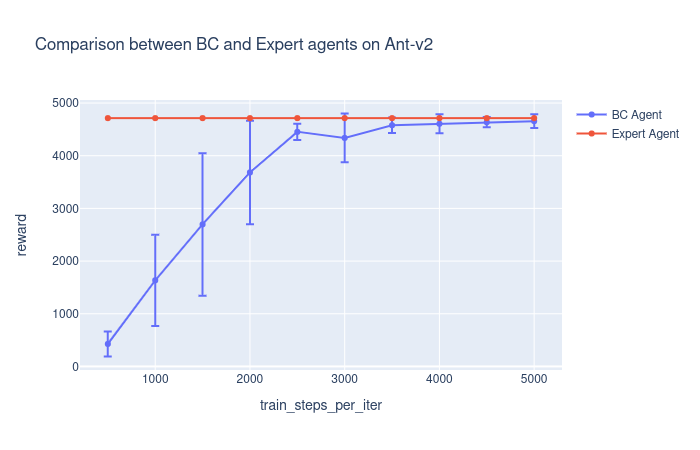
\includegraphics[scale=0.5]{./figs/comparison_bc_expert.png}
\end{center}
\caption{Comparison between Behavioral Cloning and Expert agents on Ant-v2} 
\label{fig:bcexpert}
\end{figure}

\section{Dagger}%
\label{sec:Dagger}

\begin{itemize}
    \item [2.2] \prettyref{fig:dagger} shows a fair comparison between BC,Dagger and 
    Expert agents. Using the same hyperparameters for BC on the last section, with 200000 steps training per iteration,
    the dagger has 40 iterations and 5000 steps training per iteration(Total: 200000). As we can see, dagger achieves
    performance similar to expert agent, but BC shows worse performance between them. 
\end{itemize}

\begin{figure}
\begin{center}
    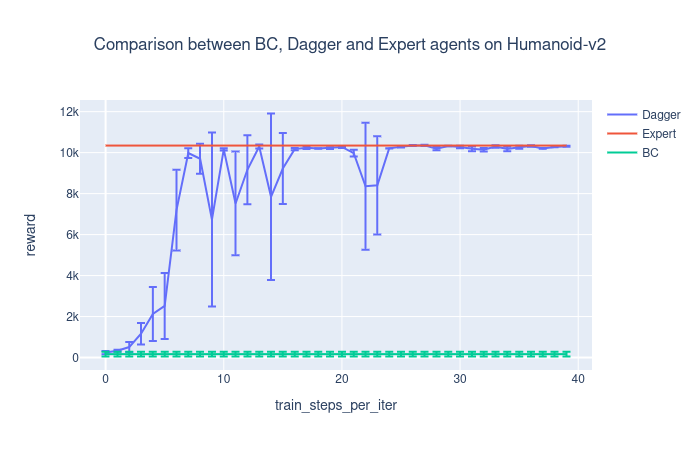
\includegraphics[scale=0.5]{./figs/comparison_bc_expert_dagger.png} 
\end{center}
\caption{Comparison between Behavioral Cloning, Expert and Dagger agents on Humanoid-v2}
\label{fig:dagger}
\end{figure}


    
\end{document}
